\section{Preliminary Models}
\subsection{Daimler Models}

%\subsubsection{Introduction}

Daimler use-case is based on two application scenarios \cite{Fer14}: i) early recognition of a lane change manoeuvre; and ii) earlier prediction of the need for a lane change based on relative dynamics between two vehicles driving in the same lane at different speeds. 

The first scenario has been previously addressed by Daimler \cite{kasper2012object}. The main result of this previous work was a static object oriented Bayesian network \cite{koller1997object} able to detect a manoeuvre 0.6s before execution. The goal now is to extend the prediction horizon for manoeuvre recognition at least 1-2 seconds to further improve the quality of the on board adaptive cruise control. As we will explain later, this improvement is expected to be achieved by a dynamic extension of this previously proposed static model. We built on this previously proposed static model for two main reasons: although with a limit prediction horizon, this static model has proven to be very robust for this task and it is considered to be the gold-standard for this problem in Daimler; and, also, because the developed models in this project are expected to be integrated in a ECU \cite{Fer14}, and the advances made about this respect for the static model \cite{Weidl2014} can be exploited during the integration in the ECU of their dynamic counterparts. 



\subsubsection{Early recognition of a lane change manoeuvre}

The basic settings of this application scenario are as follows. Let us suppose we are driving our car, which will be referred to as the EGO vehicle, in a highway. This EGO vehicle is equipped with a video camera, radar and some on-board sensors.  Using the data provided by these sensors, the challenge consists on making an early recognition of a manoeuvre either by the EGO or another relevant car in the traffic scene (OBJ). In total, the system is expected to recognise the following set of manoeuvres (a visual description of them is given below in Figure \ref{Figure:DaimlerManeuvers}):
\begin{enumerate}
\item \textbf{Object-CutIn}: A vehicle is moving to the lane where the EGO vehicle is placed.
\item \textbf{Object-CutOut}:  A vehicle that was driving in front of the EGO is leaving the EGO's lane.
\item \textbf{Object-Follow}: There is no lane change. The EGO is driving and there is some other vehicle in front.
\item \textbf{Lane-Follow}: There is no lane change. The EGO is driving and there are no other vehicles in front.
\item \textbf{EGO-CutIn}: The EGO vehicle is moving right-direction to a new lane already occupied by another vehicle. 
\item \textbf{EGO-CutOut}: The EGO vehicle is leaving left-direction the lane where it was driving.
\end{enumerate}

\begin{figure}
\begin{center}
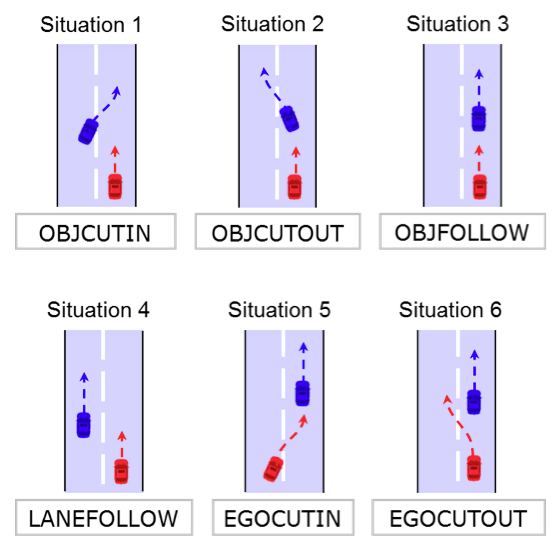
\includegraphics[scale=0.4]{./figures/DaimlerManeuvers}
\caption{\label{Figure:DaimlerManeuvers}Different maneuvers which should be identified by the AMIDST system.  Red blocks represent the EGO vehicle and blue blocks represent other vehicles in the scene.
}
\end{center}
\end{figure}

Instead of working with the raw data from the video, radar and on-board sensors, the manoeuvre recognition system uses the so-called ``object data'', which contains ``high level'' representations or features describing the ``traffic scene'' such as EGO's speed, distance between EGO and another vehicle in front, etc.  
\begin{figure}
\begin{center}
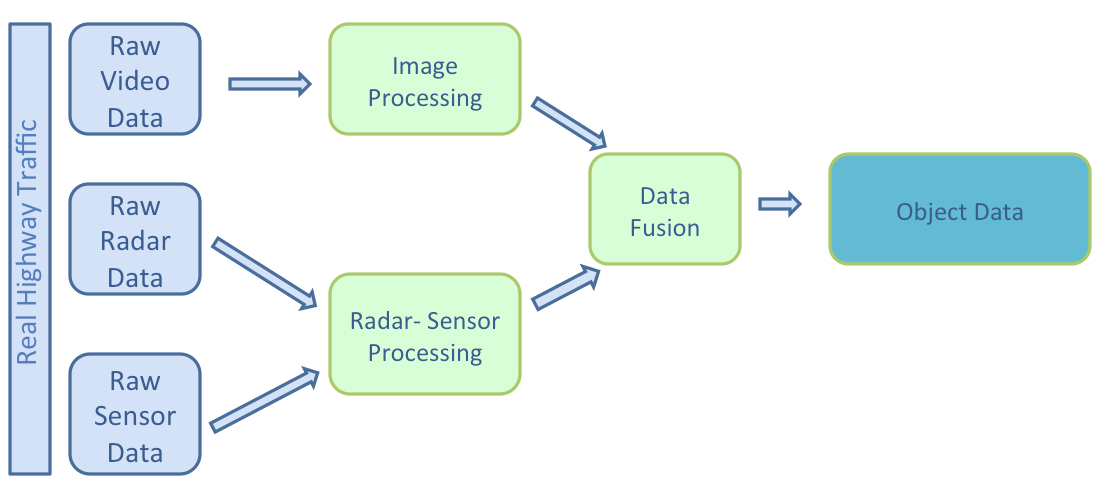
\includegraphics[scale=0.35]{./figures/DaimlerDataFlow}
\caption{\label{Figure:DaimlerDataFlow} Daimler's Data Flow.}
\end{center}
\end{figure}

Figure \ref{Figure:DaimlerDataFlow} contains a visual description of the current data flow used to create this ``object data''.  As can be seen in this figure, in a first step the raw data coming from the video, radar and sensors is preprocessed. In a second step this preprocessed data is fused and the high-level or ``object data'' describing the traffic scene is obtained. 

As commented before, using the resulting ``object data'', Daimler has developed a probabilistic graphical model \cite{kasper2012object} which is able to recognize an ongoing manoeuvre around 0.6 seconds before the manoeuvre really takes place. This probabilistic approach is based on modelling the problem in different layers as shown in Figure \ref{Figure:DaimlerHierarchicalModelling}.



\begin{figure}
\begin{center}
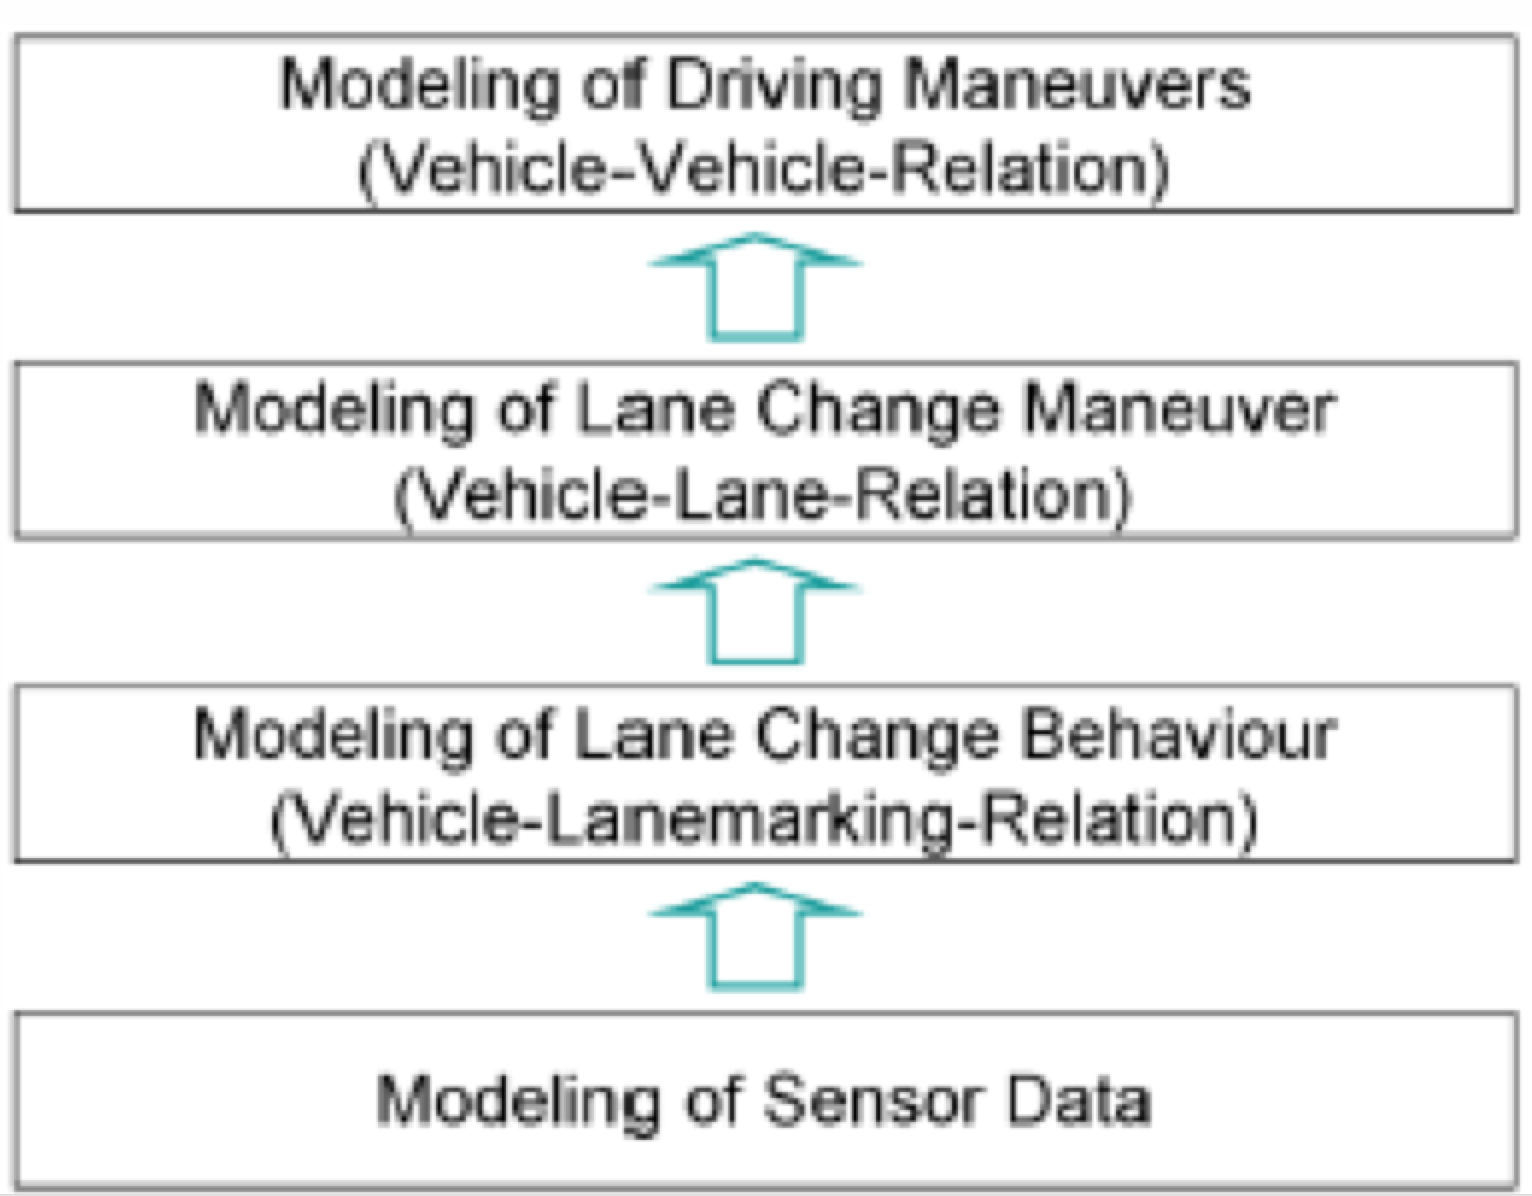
\includegraphics[scale=0.58]{./figures/DaimlerHierarchicalModelling}
\caption{\label{Figure:DaimlerHierarchicalModelling} Hierarchical layers for the recognition of driving manoeuvres.}
\end{center}
\end{figure}

The sensor data is modelled in the first step. Using this layer, a new layer is created on top with the goal of detecting a lane change behaviour. The detection of a lane change behaviour allows the system to model the lane change manoeuvre in a higher layer. Finally, with this information, the system is able to identify the kind of driving manoeuvre which is taking place between a pair of vehicles. 



\subsubsection{The static-OOBN model}

The model described here was presented in \cite{kasper2012object} as an object-oriented Bayesian network  (OOBN) \cite{koller1997object} for addressing the problem of early recognition of a lane change manoeuvre (application scenario 1).  This model works with the so-called ``object data''. This data mainly consists of a set of measured and/or computed signals or situation-features denoted by $S$ (e.g.. EGO speed, EGO lateral velocity, speed of a car in-front, etc., see \cite{kasper2012object} for further details) describing the traffic scene. The situation features used for manoeuvre recognition are structured along three main dimensions: lateral evidence (LE), trajectory (TRAJ), and occupancy schedule grid (OCCGRID).  A visual description is given in Figure \ref{Figure:DaimlerSituationFeatures}. They are referred to as the three hypotheses of possible lane change manoeuvre. The lateral evidence hypothesis considers the lateral offset and the lateral velocity of the car and accounts for the lateral movement of the car. The trajectory hypothesis tries to account for the evidence about the car's trajectory by using the measures of the angle of the car and the estimated time to crossing the line. Finally, for the occupancy grid hypothesis it is collected data that allow to identify if the surroundings of the car are going to be occupied by some other vehicle in the traffic scene. 

\begin{figure}
\begin{center}
\begin{tabular}{ccc}
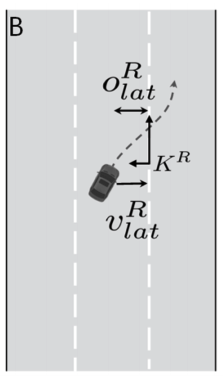
\includegraphics[scale=0.5]{./figures/DaimlerLEHipothesis} &

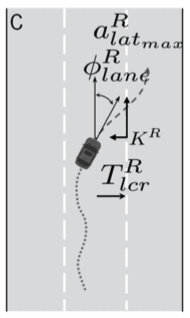
\includegraphics[scale=0.5]{./figures/DaimlerTRAJHipothesis} &

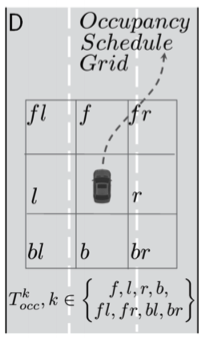
\includegraphics[scale=0.5]{./figures/DaimlerOCCGRIDHipothesis} \\

Lateral Evidence & Trajectory & Occupancy Grid \\
\end{tabular}
\caption{\label{Figure:DaimlerSituationFeatures}  The three main dimensions of the situation features \cite{kasper2012object}.}
\end{center}
\end{figure}



%The whole modelling is structured in hierarchical layers as detailed in Figure \ref{Figure:DaimlerHierarchicalModelling} and it has been previously implemented \cite{kasper2012object} using an object-%oriented Bayesian network (OOBN) \cite{koller1997object}. 
%Even using this high-level features, the modelling problem is very complex. 
%At the same time, the problem contain a lot of structure and can be divided in simpler and similar sub-problems. For example, when deciding whether there is evidence or not that a car is performing a %lateral movement to the right, we can employ two situation-features such as the lateral velocity to the right and the lateral offset w.r.t. the right lane marking of this vehicle to make this decision. But %we will find a quite similar problem when deciding about the lateral movement evidence of the EGO car or any other car, when the only difference that will use another situation-features (e.g. the right %lateral velocity of the EGO) .

The general structure of this OOBN model consists of a number of abstraction levels as detailed in Figure \ref{Figure:DaimlerOOBNAbstraction}. : 

\begin{description}
\item[Class Sensor Measurement:]  This class represents objects at the lowest level of the OOBN. It models the so-called \textit{measured data} which are  the observations characterising a situation. They are acquired from sensors and computations (see Figure \ref{Figure:DaimlerDataFlow}). The structure is the common one found in a standard Kalman filter model to account for sensor noise or fault:  S\_MEAS refers to the sensor-reading value, S\_REAL to the real value and S\_SIGMA to the uncertainty in the measurements. So, the sensor-reading of a measured variable is conditionally dependent on random changes in the real value under measurement (S\_REAL) and sensor noise/fault (S\_SIGMA).  In this problem,  and due to the particular data flow in  Daimler, observations about the measured value S\_MEAS but also about the uncertainty of the measurement S\_SIGMA are given in the object data. 

\item[Class Hypothesis:] This class is in a higher level and  directly depends on the real values S\_REAL obtained in the previous class. These real sensor values  are used to evaluate different hypothesis such as lateral evidence, trajectory and occupancy grid. 

\item[Class Event:] This class is at the top level of the modelling. It allows to model high-level hypothesis based on low-level hypothesis in a recursive way. This class also includes the variable or the event  representing the the possible traffic manoeuvres of the own and neighbour vehicles. This event is modelled based on previous high-level hypothesis. 

\end{description}

\begin{figure}
\begin{center}
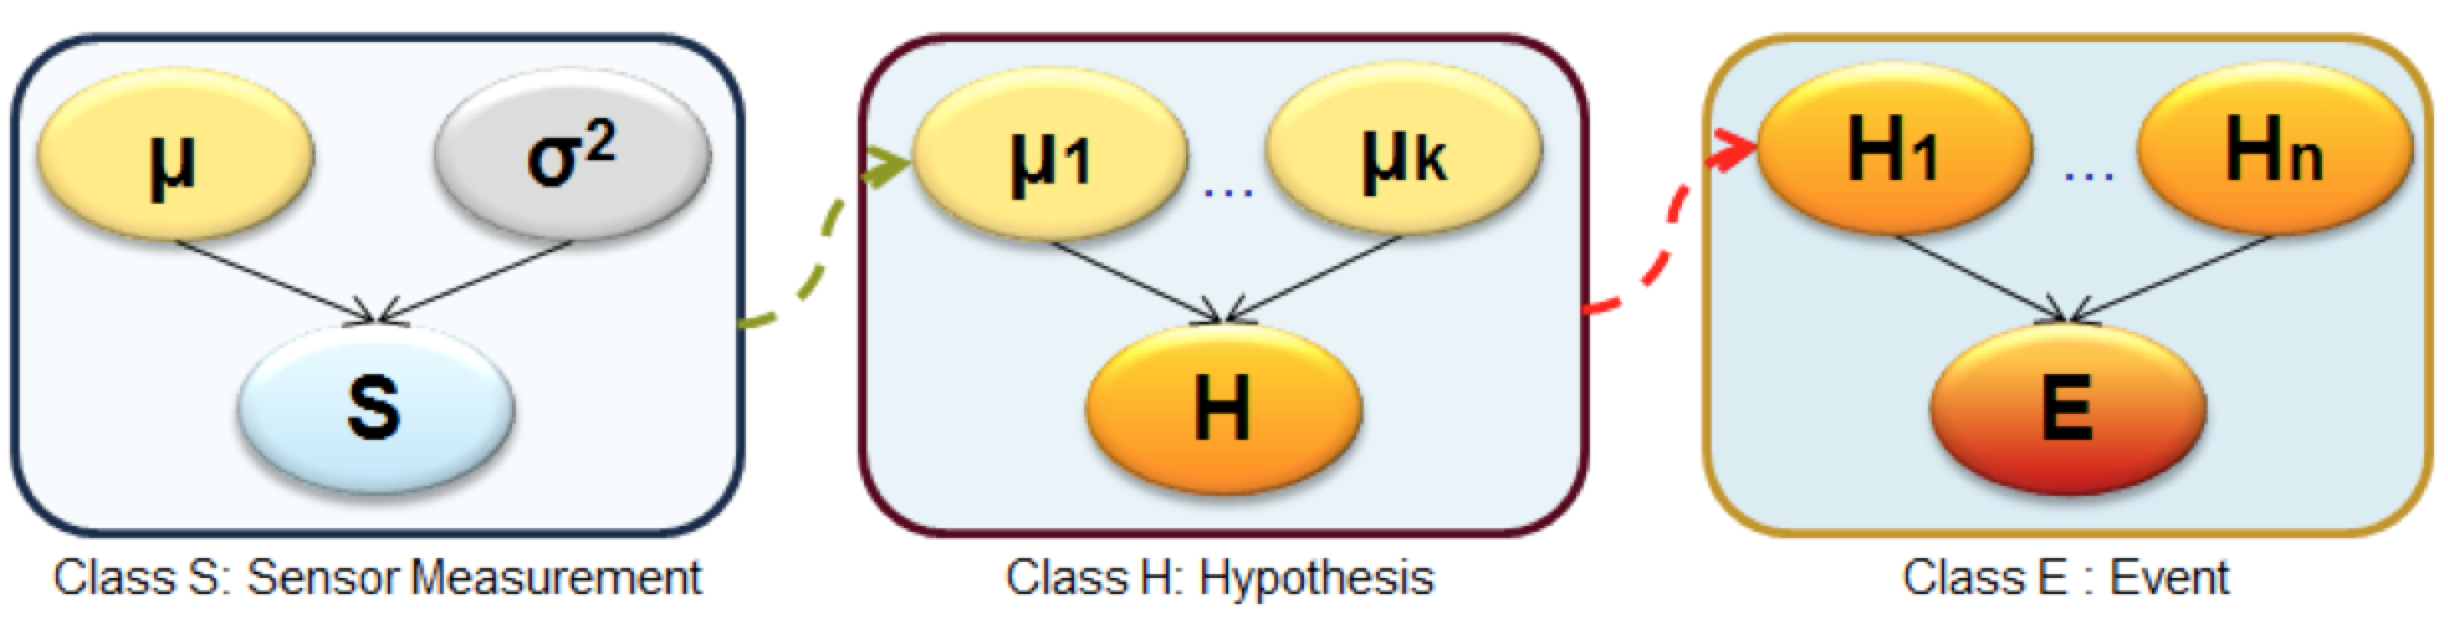
\includegraphics[scale=0.58]{./figures/DaimlerOOBNAbstraction}
\caption{\label{Figure:DaimlerOOBNAbstraction} Static-OOBN model for the prediction of an event (maneuver) \cite{Weidl2014}.}
\end{center}
\end{figure}

Finally, in Figure \ref{Figure:DaimlerLE}, we show a concrete fragment of the OOBN model related the modelling of the lateral evidence (LE) hypothesis. As can be seen, this hypothesis depends on the lateral offset to a lane marking, O\_LAT\_REAL, and on the lateral velocity, V\_LAT\_REAL, of the car. Both measures are estimated from their measured values, O\_LAT\_MEAS and V\_LAT\_MEAS, and from the estimated uncertainty of the measurement,O\_LAT\_SIGMA and O\_LAT\_SIGMA. This part the OOBN is used to model the growing probability for the lateral evidence to cross the lane marking, based on the vehicle coming closer to the lane marking and the increase of its lateral velocity.

\begin{figure}
\begin{center}
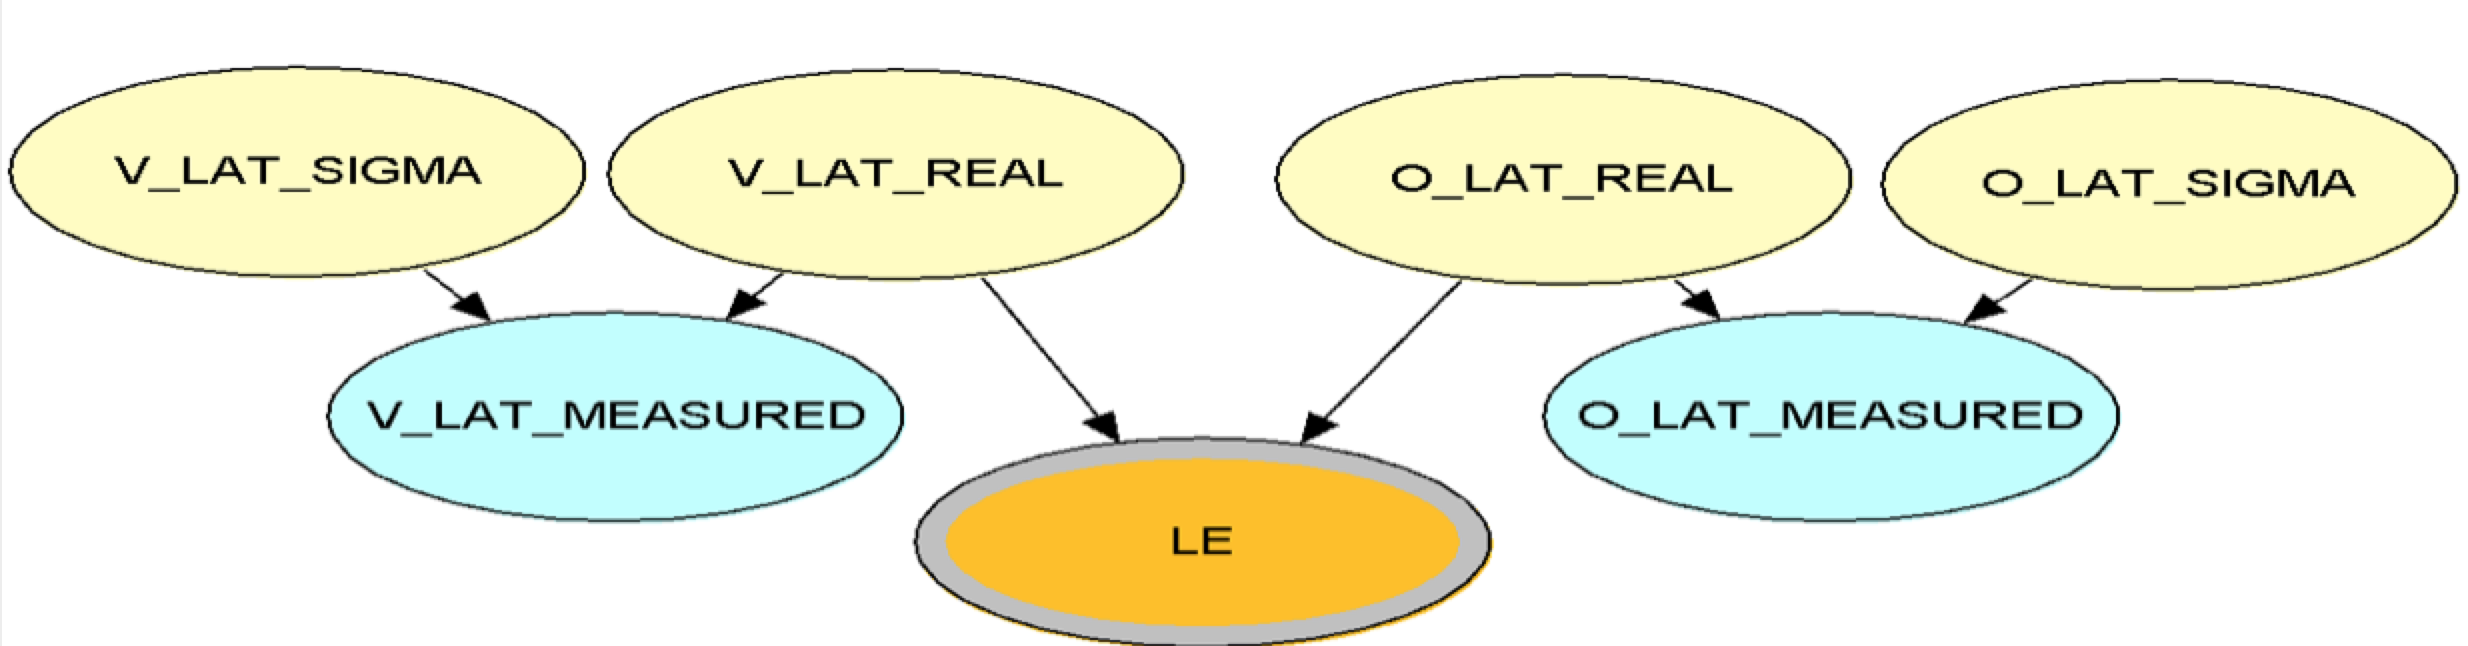
\includegraphics[scale=0.58]{./figures/DaimlerLE}
\caption{\label{Figure:DaimlerLE} Static BN fragment for the LE hypothesis.}
\end{center}
\end{figure}


As denoted in Figure \ref{DaimlerOOBNAbstraction} and \ref{Figure:DaimlerLE}, S\_REAL variables are continuous variables. However, this modelling has significant impact when making inference because we have discrete childs with continuous parents and, in consequence, the conditional probability distribution of the hypotheses given then S\_REAL variables does not fall inside the conditional linear Gaussian family \cite{nielsen2009bayesian}. One possible solution used in  \cite{kasper2012object} is to discretize the S\_REAL variables. In this case, we have that S\_MEAS, S\_SIGMA are always observed so their potentials can be collapsed/combined with the potential of the respective  discretized S\_REAL variables. Then, all the inferences in this probabilistic model can be made by only using discrete potentials \cite{nielsen2009bayesian}.

